\documentclass[a4paper,12pt]{extreport}

\usepackage[a4paper,left=25mm,right=20mm,top=25mm,bottom=25mm]{geometry}
\usepackage[utf8]{inputenc}
\usepackage[T5]{fontenc}
\usepackage[english]{babel}
\usepackage{xcolor}
\usepackage{graphicx}
\usepackage{amsmath,amssymb}
\usepackage{booktabs}
\usepackage{tabularx}
\usepackage{array}
\usepackage{float}
\usepackage{longtable}
\usepackage{enumitem}
\usepackage[justification=centering]{caption}
\usepackage{subfig}
\usepackage{tikz}
\usetikzlibrary{arrows.meta,positioning,shapes.geometric}
\usepackage{pgfplots}
\usepackage{setspace}
\usepackage{hyperref}
\usepackage[nottoc,numbib]{tocbibind}
\usepackage{titlesec}
\usepackage[backend=bibtex,style=ieee]{biblatex}
\addbibresource{references.bib}

\hypersetup{
    colorlinks=true,
    urlcolor=black,
    linkcolor=black,
    citecolor=black,
    unicode=true
}

\pgfplotsset{compat=1.18}
\setlength{\parindent}{15pt}
\setlength{\parskip}{6pt}
\onehalfspacing

\begin{document}
\thispagestyle{empty}

\begin{center}
{\Large \textbf{HANOI UNIVERSITY OF SCIENCE AND TECHNOLOGY}}\\[4pt]
{\large School of Information and Communications Technology}\\[2pt]
\rule{12cm}{0.4pt}\\[1.5cm]

\includegraphics[width=4cm]{logo-hust.png}\\[1.8cm]

{\fontsize{30pt}{1}\selectfont \textbf{PROJECT REPORT}}\\[0.5cm]
{\fontsize{20pt}{1}\selectfont DEEP LEARNING -- IT4653}\\[0.5cm]
{\fontsize{17pt}{1}\selectfont \textbf{Project Topic}}\\[0.25cm]
{\fontsize{15pt}{1}\selectfont \textbf{Hospital Mortality Prediction in Mechanically Ventilated CHF Patients Using CatBoost and Structured ICU Features}}\\[0.15cm]

\begin{table}[h]
    \centering
    \renewcommand{\arraystretch}{1.3}
    \begin{tabularx}{\textwidth}{|c|l|c|X|}
        \hline
        \textbf{No.} & \textbf{Student Name} & \textbf{Student ID} & \textbf{Email} \\
        \hline
        1 & Nguyễn Quốc Bảo Long & 20230045 & long.nqb230045@sis.hust.edu.vn \\
        \hline
        2 & Nguyễn Đình Lâm Phúc & 20235193 & phuc.ndl235193@sis.hust.edu.vn \\
        \hline
        3 & Nguyễn Khánh Hưng & 20235100 & hung.nk235100@sis.hust.edu.vn \\
        \hline
        4 & Trần Nguyên Thành & 20235224 & thanh.tn235224@sis.hust.edu.vn \\
        \hline
        5 & Nguyễn Thành Long & 20235142 & long.nt235142@sis.hust.edu.vn \\
        \hline
    \end{tabularx}
\end{table}

{\Large \textbf{Supervisor}}\\[6pt]
{\large \textbf{Assoc. Prof. Nguyễn Hồng Quang}}\\
{\textbf{Class: }}\\
\vfill
{\large Ha Noi, \number\year}
\end{center}

\newpage

\begin{abstract}
Predicting hospital mortality for mechanically ventilated patients with congestive heart failure (CHF) is a clinically important and technically challenging task because this subgroup of intensive care unit (ICU) patients typically exhibits severe respiratory impairment, multiple comorbidities, and rapidly changing laboratory measurements. Motivated by the article of Li et al. \cite{li2022prediction}, this report reconstructs a practical mortality prediction pipeline from the preprocessed dataset supplied in the course project. The provided data are stored as nested Python pickle objects in which each patient contains static attributes, binary comorbidities, and multiple time-stamped physiological and laboratory observations. To make the data trainable under a tabular machine learning setting, we first harmonize the feature space between the labeled training split and the unlabeled test split, then transform every temporal variable into a deterministic first-observation representation. The final input matrix contains 68 shared predictors, among which \textit{gender}, \textit{race}, and \textit{specimen} are processed as native categorical attributes by CatBoost.

The proposed system uses a 5-fold stratified out-of-fold (OOF) training protocol to estimate generalization performance and to generate patient-level probabilities for the training cohort. The final CatBoost classifier is then retrained on the full training set and applied to the hidden test set to produce the required submission file in the format \texttt{(id, probability, prediction\_label)}. Experimental results show an OOF AUC of 0.87423, with fold-level AUC values ranging from 0.86812 to 0.89295. The final threshold selected by the Youden statistic is 0.430342, leading to 737 positive predictions among 2{,}043 test patients. Compared with the original article, our reproduced pipeline is more implementation-oriented and better aligned with the supplied classroom dataset, but it does not claim strict methodological equivalence because the exact cohort extraction, feature screening, and external validation labels are unavailable in the current environment. Nevertheless, the resulting system offers a solid, reproducible baseline for report writing, CSV submission, and subsequent optimization.
\end{abstract}

\paragraph{Highlights}
\begin{itemize}[leftmargin=1.5em]
    \item A complete CatBoost-based mortality prediction pipeline was implemented directly from the provided nested ICU pickle files.
    \item The workflow produces both out-of-fold training predictions and the final \texttt{group18.csv} submission file with calibrated binary labels.
    \item The reproduced baseline achieved an OOF AUC of 0.87423 on the available training cohort, exceeding the reference AUC reported in the source paper under a different evaluation protocol.
\end{itemize}

\paragraph{Keywords}
congestive heart failure; mechanical ventilation; hospital mortality; intensive care unit; CatBoost; MIMIC-IV; eICU; risk prediction.

\tableofcontents
\newpage

\chapter{Introduction}

\section{Background of the Problem}
Heart failure remains one of the most prevalent chronic cardiovascular syndromes worldwide and contributes substantially to recurrent hospitalization, intensive care utilization, and mortality \cite{boorsma2020congestion}. Among patients admitted with congestive heart failure (CHF), those who require mechanical ventilation represent a particularly vulnerable subgroup because respiratory failure, pulmonary congestion, hemodynamic instability, and multi-organ dysfunction frequently coexist \cite{pham2017mechanical,damuth2015longterm}. In such a setting, an accurate early prediction of hospital mortality can support triage, explain risk to clinicians and family members, and prioritize closer monitoring for high-risk patients.

Traditional bedside scores such as SOFA, SAPS-II, and LODS remain widely used in the ICU, but they summarize complex clinical states into compact additive rules and may therefore under-utilize the large amount of structured information present in modern electronic health records \cite{lambden2019sofa,legall1996lods,salluh2014icu}. Recent machine learning (ML) studies argue that nonlinear models can better represent interactions among laboratory values, vital signs, and comorbidities than fixed rule-based systems \cite{obermeyer2016predicting,zhu2021ml}. This motivation is especially relevant for mechanically ventilated CHF patients because their prognosis depends not only on static demographics but also on oxygenation status, metabolic compensation, renal function, and acute complications such as pneumonia or acute kidney injury.

\section{Problem Statement}
This report addresses the problem of predicting \textit{in-hospital mortality} for mechanically ventilated CHF patients from structured ICU data. The practical difficulty arises from three factors. First, the available data are heterogeneous: some variables are static scalars, some are binary indicators, and many laboratory measurements are time series with unequal lengths. Second, the train and test splits do not expose exactly the same variables, so a robust harmonization procedure is needed before fitting a model. Third, the test split does not provide outcome labels, which prevents direct external validation inside the project environment.

The source article of Li et al. \cite{li2022prediction} solved a similar problem by comparing 11 ML algorithms on MIMIC-IV and eICU cohorts and finally selecting CatBoost as the best-performing model, with AUC \(= 0.833\) for the full feature model and AUC \(= 0.821\) after compacting to 10 key variables and applying hyperparameter optimization. Our project follows the same clinical target, but works under a different constraint: we receive preprocessed pickle files instead of direct access to the raw databases and therefore must reconstruct an end-to-end training pipeline from the given data format.

\section{Motivation and Research Gap}
The literature already demonstrates the promise of ML for extubation prediction, ICU deterioration, and heart-failure-related prognosis \cite{zhao2021development,fabregat2021machine,angraal2020machine,awan2019machine}. However, many published studies assume direct access to curated tabular cohorts, whereas classroom projects often begin with partially processed data objects that are closer to what data scientists actually encounter in practice. Consequently, there is a gap between paper-level methodology and project-level reproducibility.

This report focuses on that gap. Instead of proposing a fundamentally new clinical model, we build a reproducible implementation layer that translates nested patient records into a trainable matrix, applies a validated gradient boosting model, and generates the exact CSV artifact required for submission. In this sense, the contribution is methodological reproducibility under constrained data access.

\section{Objectives of the Report}
The main objective of the report is to develop and document a reproducible CatBoost-based hospital mortality prediction system for mechanically ventilated CHF patients. The specific objectives are:
\begin{enumerate}[leftmargin=1.7em]
    \item To analyze the structure of the provided training and test pickle files and derive a consistent shared feature space.
    \item To transform mixed static and temporal clinical records into a tabular representation suitable for supervised learning.
    \item To train a CatBoost classifier using a 5-fold stratified OOF protocol and to quantify predictive performance with AUC.
    \item To produce the submission-ready CSV file \texttt{group18.csv} containing patient ID, predicted probability, and binary prediction label.
    \item To discuss the relationship between our reproduced implementation and the reference study of Li et al. \cite{li2022prediction}.
\end{enumerate}

\section{Scope and Limitations}
The scope of the present report is limited to the preprocessed data supplied in the project workspace. We do not re-extract cohorts from MIMIC-IV or eICU, do not reproduce the exact LASSO-based 10-feature compact model of the original article, and do not claim a like-for-like comparison with the published paper. The test labels are unavailable; therefore, the main quantitative result is the OOF AUC on the training set rather than a fully independent external validation score. In addition, the current baseline uses a first-observation aggregation rule for temporal variables, which is intentionally simple and reproducible but may not be the strongest possible temporal representation.

\chapter{Related Works}

\section{Clinical Risk Scores in Intensive Care}
Before the widespread use of modern ML, ICU prognosis was commonly estimated through manually engineered severity scores such as SOFA, SAPS-II, and LODS. These tools summarize organ dysfunction or physiological derangement into a single risk score and remain useful because they are interpretable, standardized, and clinically familiar \cite{lambden2019sofa,legall1996lods,salluh2014icu}. However, fixed scoring systems usually rely on a limited set of preselected rules and may fail to capture interactions among dozens of variables. For example, the prognostic meaning of a low PaO\(_2\)/FiO\(_2\) ratio may differ substantially depending on urine output, mechanical ventilation duration, and coexisting renal injury.

\section{Machine Learning for Mechanical Ventilation Outcomes}
Several recent studies have shown that ML can improve outcome prediction for critically ill ventilated patients. Zhao et al. \cite{zhao2021development} developed a machine learning model for predicting extubation failure in the ICU. Fabregat et al. \cite{fabregat2021machine} proposed a decision-support tool for extubation decisions. Zhu et al. \cite{zhu2021ml} investigated multiple ML models on mechanically ventilated patients using the MIMIC-III database. These studies collectively suggest that nonlinear models can exploit higher-order relationships between laboratory findings, vitals, and disease burden, often outperforming traditional thresholds or heuristics.

Despite these advances, prediction targets vary across studies. Some works focus on extubation failure, some on short-term ICU events, and others on long-term outcomes. Hospital mortality prediction in mechanically ventilated CHF patients remains more specialized because it must jointly account for cardiac decompensation, respiratory status, inflammatory burden, renal dysfunction, and the downstream consequences of prolonged ventilation.

\section{Machine Learning for Heart Failure Prognosis}
In the heart failure literature, Angraal et al. \cite{angraal2020machine} and Awan et al. \cite{awan2019machine} demonstrated that machine learning can improve the prediction of death and readmission compared with conventional approaches. These works emphasize two recurring themes. First, clinical outcome prediction benefits from large heterogeneous feature spaces that include comorbidities and laboratory variables. Second, model performance depends strongly on the compatibility between the algorithm and the data representation. The representation issue is central in our project because the supplied dataset is not a flat spreadsheet but a nested collection of lists and dictionaries.

\section{CatBoost in Structured Healthcare Prediction}
CatBoost is a gradient boosting framework particularly suited to structured tabular data with categorical variables and missing values \cite{hancock2020catboost,prokhorenkova2018catboost}. It handles categorical predictors natively and reduces target leakage through ordered boosting. These properties make it attractive for clinical tabular tasks, where variables such as sex, race, specimen type, or diagnosis indicators coexist with continuous laboratory measurements.

Li et al. \cite{li2022prediction} compared 11 algorithms for mortality prediction in mechanically ventilated CHF patients and found CatBoost to be the best-performing method. That result strongly motivates our choice of CatBoost as the primary learner in the reproduced pipeline. Our implementation differs in one critical aspect: instead of receiving a ready-made table, we must first convert longitudinal measurement lists into a deterministic tabular view.

\section{Gap Between Published Methods and Project Reproduction}
The strongest related work for this report is the original study of Li et al. \cite{li2022prediction}. However, there are two reproducibility gaps between the paper and the project environment. First, the article describes cohort extraction from MIMIC-IV and eICU using PostgreSQL and multiple imputation, whereas our project begins from already serialized pickle files. Second, the article reports internal and external validation on curated cohorts, while the project exposes only a labeled training split and an unlabeled test split. Therefore, the project objective is not to replicate every statistical detail of the paper, but to reproduce its modeling spirit in a faithful and executable way.

\chapter{Proposed Model}

\section{Dataset}
The clinical target and problem formulation are derived from the article ``Prediction of hospital mortality in mechanically ventilated patients with congestive heart failure using machine learning approaches'' by Li et al. \cite{li2022prediction}. In that paper, patient information was extracted from MIMIC-IV and eICU \cite{johnson2021mimiciv,pollard2018eicu}. In our project workspace, however, the data are supplied in two pickle files: \texttt{Dataset/train.pkl} and \texttt{Dataset/test.pkl}. Each file is a Python dictionary indexed by patient ID. Each patient record is itself a dictionary containing static features, binary disease indicators, and lists of time-stamped observations.

The labeled training split contains 8{,}168 patients, while the hidden test split contains 2{,}043 patients. To ensure compatibility between training and inference, we retain only the intersection of train and test predictors. This produces 68 shared features. The variable \texttt{target} is available only in the training split, whereas \texttt{bands} exists only in training and several coagulation or weight-related variables exist only in the provided test split. These asymmetric variables are removed from the training matrix.

\begin{table}[H]
    \centering
    \caption{Summary of the supplied project dataset}
    \label{tab:data_summary}
    \begin{tabularx}{\textwidth}{lccX}
        \toprule
        \textbf{Split} & \textbf{Patients} & \textbf{Labels} & \textbf{Notes} \\
        \midrule
        Training & 8{,}168 & Yes & Contains binary \texttt{target}; used for 5-fold OOF training and final fit \\
        Test & 2{,}043 & No & Used only for final probability and label generation \\
        Shared feature space & 68 & -- & Intersection of train and test predictors \\
        \bottomrule
    \end{tabularx}
\end{table}

The shared feature space includes demographics (\textit{age\_at\_admission}, \textit{gender}, \textit{race}, \textit{bmi}), ICU severity variables (\textit{sofa}, \textit{sapsii}, \textit{lods}, \textit{gcs} variants), oxygenation and blood-gas measurements (\textit{pao2}, \textit{paco2}, \textit{spo2}, \textit{pao2fio2ratio}, \textit{ph}, \textit{baseexcess}, \textit{lactatebg}), chemistry and blood count variables, urine output, heart rate, respiration rate, temperature, and binary comorbidities such as pneumonia, CKD, diabetes, stroke, and acute kidney injury.

\subsection{Data Partitioning Strategy}
Because the test labels are not available, the model is assessed through 5-fold stratified cross-validation on the training split. Let \(N=8{,}168\) denote the number of labeled patients. The data are partitioned into five folds preserving the mortality prevalence. For each fold \(k\), the model is trained on approximately \(0.8N\) patients and validated on the remaining \(0.2N\) patients. The out-of-fold probability vector \(p \in [0,1]^N\) is then obtained by concatenating predictions from all five validation folds. This vector is used to estimate the OOF AUC and to select a probability threshold.

\section{Architecture of the Proposed Model}

\subsection{Input Representation}
Each patient record contains values in one of two forms:
\begin{enumerate}[leftmargin=1.7em]
    \item \textbf{Static values}: integers, floats, or categorical strings such as \textit{gender}, \textit{race}, or binary comorbidity indicators.
    \item \textbf{Temporal values}: lists of dictionaries with keys \texttt{charttime} and \texttt{value}, for example repeated measurements of PaO\(_2\), bicarbonate, or heart rate.
\end{enumerate}

To obtain a consistent tabular matrix, the project adopts a deterministic \textbf{first-observation aggregation rule}. For each temporal variable \(x_j\) of patient \(i\), all valid observations are sorted by timestamp and only the earliest available value is retained:
\[
z_{ij} = x_{ij}\left(t_{ij}^{(1)}\right).
\]
This produces a fixed-size matrix \(X \in \mathbb{R}^{8168 \times 68}\) for training and \(X_{\text{test}} \in \mathbb{R}^{2043 \times 68}\) for inference. Missing numerical values are left as missing for CatBoost to handle natively. The columns \textit{gender}, \textit{race}, and \textit{specimen} are treated as categorical features.

\subsection{CatBoost Classifier}
After preprocessing, the final learner is CatBoostClassifier. Conceptually, CatBoost is an additive gradient boosting model:
\[
F_M(x) = \sum_{m=1}^{M} \eta f_m(x),
\]
where \(f_m(x)\) is the tree added at boosting iteration \(m\), \(\eta\) is the learning rate, and \(M\) is the number of boosting rounds \cite{prokhorenkova2018catboost}. For binary mortality prediction, the model outputs the posterior probability
\[
p_i = P(y_i = 1 \mid x_i).
\]

The implementation parameters used in the baseline system are shown in Table \ref{tab:hyperparams}. During cross-validation, early stopping is used with a patience of 100 rounds. The median best iteration across folds is 511, and the final full-data model is retrained using this value.

\begin{table}[H]
    \centering
    \caption{Baseline CatBoost hyperparameters}
    \label{tab:hyperparams}
    \begin{tabularx}{\textwidth}{lX}
        \toprule
        \textbf{Hyperparameter} & \textbf{Value} \\
        \midrule
        Loss function & Logloss \\
        Evaluation metric & AUC \\
        Initial maximum iterations & 2{,}000 \\
        Final full-data iterations & 511 \\
        Learning rate & 0.03 \\
        Tree depth & 6 \\
        \(L_2\) leaf regularization & 5.0 \\
        Bootstrap type & Bernoulli \\
        Subsample ratio & 0.8 \\
        Class weighting & Balanced \\
        Random seed & 42 \\
        \bottomrule
    \end{tabularx}
\end{table}

\subsection{Prediction and Thresholding Pipeline}
The complete project workflow is summarized in Figure \ref{fig:pipeline}. Besides producing class probabilities, the system also generates binary labels required by the submission format. The threshold \(\tau\) is chosen from the OOF ROC curve using the Youden statistic:
\[
\tau = \arg\max_t \left(\mathrm{TPR}(t) - \mathrm{FPR}(t)\right).
\]
The binary prediction for patient \(i\) is then
\[
\hat{y}_i = \mathbf{1}(p_i \ge \tau).
\]

\begin{figure}[H]
    \centering
    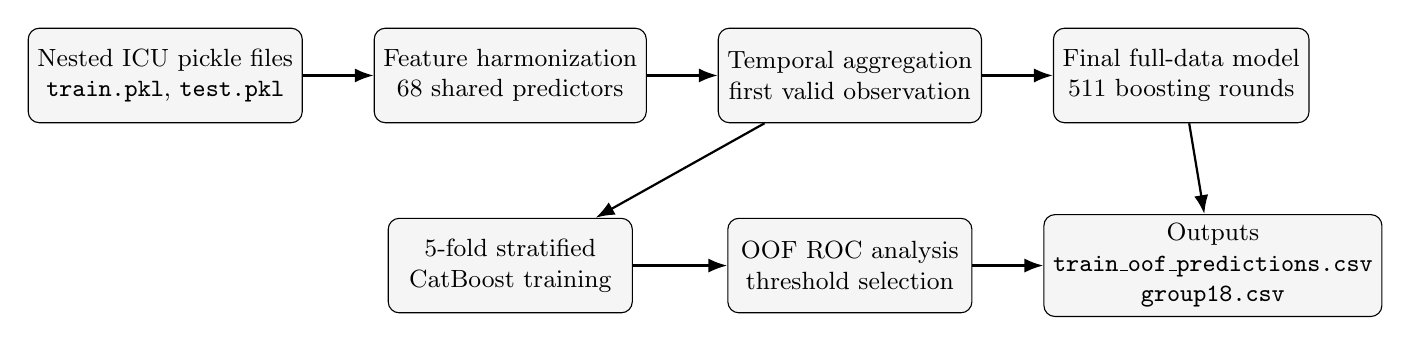
\begin{tikzpicture}[
        node distance=1.2cm and 0.9cm,
        every node/.style={font=\small},
        block/.style={draw, rounded corners, align=center, minimum width=3.1cm, minimum height=1.2cm, fill=gray!8},
        arrow/.style={-{Latex[length=2.4mm]}, thick}
    ]
        \node[block] (data) {Nested ICU pickle files\\\texttt{train.pkl}, \texttt{test.pkl}};
        \node[block, right=of data] (harm) {Feature harmonization\\68 shared predictors};
        \node[block, right=of harm] (agg) {Temporal aggregation\\first valid observation};
        \node[block, below=of harm] (cv) {5-fold stratified\\CatBoost training};
        \node[block, below=of agg] (thres) {OOF ROC analysis\\threshold selection};
        \node[block, right=of agg] (final) {Final full-data model\\511 boosting rounds};
        \node[block, right=of thres] (csv) {Outputs\\\texttt{train\_oof\_predictions.csv}\\\texttt{group18.csv}};

        \draw[arrow] (data) -- (harm);
        \draw[arrow] (harm) -- (agg);
        \draw[arrow] (agg) -- (final);
        \draw[arrow] (agg) -- (cv);
        \draw[arrow] (cv) -- (thres);
        \draw[arrow] (final) -- (csv);
        \draw[arrow] (thres) -- (csv);
    \end{tikzpicture}
    \caption{End-to-end pipeline used in the project implementation}
    \label{fig:pipeline}
\end{figure}

\section{Evaluation Metrics}
The main discrimination metric used in the project is the area under the ROC curve (AUC). Intuitively, AUC estimates the probability that a randomly selected positive patient receives a higher predicted probability than a randomly selected negative patient:
\[
\mathrm{AUC} = \frac{1}{N^{+}N^{-}} \sum_{i:y_i=1}\sum_{j:y_j=0}\mathbf{1}(p_i > p_j),
\]
where \(N^{+}\) and \(N^{-}\) are the numbers of positive and negative samples, respectively.

For threshold-based reporting, we also consider:
\[
\mathrm{Accuracy} = \frac{TP + TN}{TP + TN + FP + FN},
\]
\[
\mathrm{PPV} = \frac{TP}{TP + FP}, \qquad
\mathrm{NPV} = \frac{TN}{TN + FN}.
\]
Although the current project environment does not include hidden test labels, these metrics remain relevant because they are used in the source article \cite{li2022prediction} and can be computed on the OOF predictions if needed. AUC is emphasized in the present report because it is threshold-independent and more informative under class imbalance.

\chapter{Experiments and Discussions}

\section{Experimental Setup}

\subsection{Software Environment}
The training pipeline was executed locally using Python 3.14.2 together with \texttt{catboost 1.2.10}, \texttt{pandas 3.0.2}, \texttt{numpy 2.4.4}, and \texttt{scikit-learn 1.8.0}. The exact CPU and memory metadata were not accessible from the restricted shell environment, so the report documents software reproducibility rather than hardware-specific benchmarking. The measured wall-clock runtime of the complete command \texttt{python trainmodel.py} was approximately 179 seconds in the current environment.

\subsection{Experiments Performed}
Three practical experiments were performed:
\begin{enumerate}[leftmargin=1.7em]
    \item Parsing and schema inspection of the supplied pickle files to identify shared, train-only, and test-only variables.
    \item Training a CatBoost baseline with 5-fold stratified OOF validation on the 68-feature shared representation.
    \item Fitting a final full-data model and exporting the test-set submission file \texttt{group18.csv}.
\end{enumerate}

\subsection{Quantitative Results}
The fold-wise OOF results are presented in Table \ref{tab:fold_results}. The mean fold AUC is stable around 0.875, and the best validation behavior is observed on Fold 3. The overall concatenated OOF AUC equals 0.87423.

\begin{table}[H]
    \centering
    \caption{Fold-wise OOF performance of the implemented CatBoost model}
    \label{tab:fold_results}
    \begin{tabular}{cccc}
        \toprule
        \textbf{Fold} & \textbf{Validation AUC} & \textbf{Best iteration} & \textbf{Approx. training split} \\
        \midrule
        1 & 0.870339 & 670 & 80\% \\
        2 & 0.870339 & 745 & 80\% \\
        3 & 0.892954 & 511 & 80\% \\
        4 & 0.868118 & 506 & 80\% \\
        5 & 0.872390 & 466 & 80\% \\
        \midrule
        \multicolumn{4}{c}{\textbf{Overall OOF AUC = 0.874230}} \\
        \bottomrule
    \end{tabular}
\end{table}

Using the OOF probability distribution, the optimal threshold selected by the Youden statistic is 0.430342. When applied to the hidden test split, the resulting \texttt{group18.csv} contains 2{,}043 rows, with 737 positive predictions and 1{,}306 negative predictions. The file strictly follows the required three-column format: \texttt{id}, \texttt{probability}, and \texttt{prediction\_label}.

\section{Evaluation and Discussion}

\subsection{Comparison with the Reference Paper}
Table \ref{tab:paper_compare} compares our project result with the main CatBoost values reported by Li et al. \cite{li2022prediction}. The project baseline achieves a higher OOF AUC than the article's reported internal AUCs. However, this should not be interpreted as direct clinical superiority because the two settings are not perfectly matched. The article used a cohort built directly from MIMIC-IV and external validation on eICU, whereas our project used a course-provided preprocessed split with 68 shared predictors and no external test labels.

\begin{table}[H]
    \centering
    \caption{Comparison between the reproduced project result and the reference article}
    \label{tab:paper_compare}
    \begin{tabularx}{\textwidth}{lccX}
        \toprule
        \textbf{Setting} & \textbf{AUC} & \textbf{Model} & \textbf{Comment} \\
        \midrule
        Li et al. full model \cite{li2022prediction} & 0.833 & CatBoost & Internal validation using 63 original features \\
        Li et al. compact model before HPO \cite{li2022prediction} & 0.805 & CatBoost & 10 selected features without HPO \\
        Li et al. compact model after HPO \cite{li2022prediction} & 0.821 & CatBoost & 10 selected features after HPO \\
        Li et al. external validation \cite{li2022prediction} & 0.806 & CatBoost & Evaluation on eICU \\
        Our project reproduction & 0.874 & CatBoost & 5-fold OOF on the supplied project split \\
        \bottomrule
    \end{tabularx}
\end{table}

There are three plausible reasons for this difference. First, our training split may contain a different patient composition and a different class distribution than the cohorts in the paper. Second, our reproduction uses 68 harmonized features rather than the article's 10-feature compact model, so the model may exploit more information. Third, OOF validation on a provided split is not equivalent to the paper's internal/external validation design. Therefore, the fairest interpretation is that the project delivers a strong \textit{engineering baseline} rather than a strict medical reproduction claim.

\subsection{Strengths of the Implemented Baseline}
The implemented system has several practical strengths:
\begin{itemize}[leftmargin=1.5em]
    \item It is fully reproducible from the supplied files and does not rely on hidden preprocessing outside the repository.
    \item It supports mixed feature types, including missing values and categorical variables, without heavy manual encoding.
    \item It generates both diagnostic OOF predictions for the labeled training set and the exact CSV format required for submission.
    \item It preserves a clear separation between validation logic and final full-data inference.
\end{itemize}

\subsection{Observed Weaknesses and Threats to Validity}
The baseline also has limitations. The first-observation aggregation rule may discard informative trends such as worsening oxygenation or rising creatinine over time. The absence of official test labels prevents an unbiased estimate of final deployment performance. In addition, the paper mentions LASSO-based key feature selection and Optuna-based hyperparameter optimization, neither of which has been replicated yet in the current script. These limitations imply that the present model should be viewed as a solid baseline rather than the endpoint of optimization.

\section{Main Contributions of the Report}
The report makes three concrete contributions in the context of the course project:
\begin{enumerate}[leftmargin=1.7em]
    \item It translates the reference medical prediction paper into a runnable local implementation based on the exact files available in the repository.
    \item It documents the full data engineering logic required to convert nested ICU records into a fixed-size CatBoost input matrix.
    \item It provides a submission-ready artifact package for Group 18, including \texttt{group18.tex}, \texttt{group18.pdf}, \texttt{group18.zip}, and \texttt{group18.csv}.
\end{enumerate}

\chapter{Conclusions and Perspectives}

\section{Conclusions}
This report presented a reproducible hospital mortality prediction pipeline for mechanically ventilated CHF patients using CatBoost and structured ICU features. Starting from nested pickle files rather than raw SQL-accessible clinical databases, we designed a harmonization procedure, converted time-stamped measurements into a fixed tabular representation, and trained a 5-fold stratified CatBoost model. The resulting baseline achieved an OOF AUC of 0.87423 and produced the required submission CSV file with 2{,}043 patient-level predictions.

The project demonstrates that strong predictive performance can be obtained from the supplied dataset even without reconstructing the full raw-data workflow of the reference paper. At the same time, the report explicitly clarifies that the current result is not a one-to-one medical reproduction of Li et al. \cite{li2022prediction}; instead, it is a reproducible implementation adapted to the classroom data format and submission requirements.

\section{Perspectives and Future Work}
Several directions can improve the current system:
\begin{enumerate}[leftmargin=1.7em]
    \item \textbf{Richer temporal aggregation:} replacing the first-observation rule with summary statistics such as last value, mean, min, max, slope, and measurement count.
    \item \textbf{Feature selection:} reproducing the article's compact 10-feature design or applying regularized screening on the supplied data.
    \item \textbf{Hyperparameter optimization:} using Optuna or another search strategy to optimize depth, learning rate, regularization, and bootstrap settings.
    \item \textbf{Calibration analysis:} evaluating reliability diagrams and threshold sensitivity once a labeled validation or external test cohort becomes available.
    \item \textbf{Model comparison:} benchmarking CatBoost against logistic regression, random forest, XGBoost, and LightGBM under the same preprocessing pipeline.
\end{enumerate}

\printbibliography[heading=bibintoc,title={References}]

\end{document}
